\documentclass[hidelinks]{article}
\usepackage[english]{babel} 
\usepackage[utf8x]{inputenc}
%% Hyperlinks 
\usepackage{hyperref}
\hypersetup{
    colorlinks,
    linkcolor={red!50!black},
    citecolor={blue!50!black},
    linktoc=all,
    urlcolor={blue!80!black}
}
%% Graphics
\usepackage{graphicx}
\usepackage{float}

\usepackage{enumerate}
\usepackage{multicol}
% Math packages
\usepackage{amsmath}
\usepackage{amssymb}

% Algorithms
\usepackage{algorithm}
\usepackage[noend]{algpseudocode}
\newcommand\Let[2]{\State #1 $\gets$ #2}
\algrenewcomment[1]{\(\qquad \triangleright\) #1}
\newcommand\Blet[2]{\State \textbf{let} #1 \textbf{be} #2}
\errorcontextlines\maxdimen
% begin vertical rule patch for algorithmicx
% borrowing from http://tex.stackexchange.com/questions/41956/marking-conditional-versions-with-line-in-margin
% see http://tex.stackexchange.com/questions/110431/ploblems-with-vertical-lines-in-algorithmicx
\RequirePackage{zref-abspage}
\RequirePackage{zref-user}
\RequirePackage{tikz}
%\RequirePackage{atbegshi}
%\usetikzlibrary{calc}
\RequirePackage{tikzpagenodes}
\RequirePackage{etoolbox}
\makeatletter
\newcommand*\ALG@lastblockb{b}
\newcommand*\ALG@lastblocke{e}
\apptocmd{\ALG@beginblock}{%
    %\typeout{beginning block, nesting level \theALG@nested, line \arabic{ALG@line}}%
    \ifx\ALG@lastblock\ALG@lastblockb
        \ifnum\theALG@nested>1\relax\expandafter\@firstoftwo\else\expandafter\@secondoftwo\fi{\ALG@tikzborder}{}%
    \fi
    \let\ALG@lastblock\ALG@lastblockb%
}{}{\errmessage{failed to patch}}

\pretocmd{\ALG@endblock}{%
    %\typeout{ending block, nesting level \theALG@nested, line \arabic{ALG@line}}%
    \ifx\ALG@lastblock\ALG@lastblocke
        \addtocounter{ALG@nested}{1}%
        \addtolength\ALG@tlm{\csname ALG@ind@\theALG@nested\endcsname}%
        \ifnum\theALG@nested>1\relax\expandafter\@firstoftwo\else\expandafter\@secondoftwo\fi{\endALG@tikzborder}{}%
        \addtolength\ALG@tlm{-\csname ALG@ind@\theALG@nested\endcsname}%
        \addtocounter{ALG@nested}{-1}%
    \fi
    \let\ALG@lastblock\ALG@lastblocke%
}{}{\errmessage{failed to patch}}
\tikzset{ALG@tikzborder/.style={line width=0.5pt,black}}
\newcommand*\currenttextarea{current page text area}
\newcommand*{\updatecurrenttextarea}{%
    \if@twocolumn
        \if@firstcolumn
            \renewcommand*{\currenttextarea}{current page column 1 area}%
        \else
            \renewcommand*{\currenttextarea}{current page column 2 area}%
        \fi
    \else
        \renewcommand*\currenttextarea{current page text area}%
    \fi
}
\newcounter{ALG@tikzborder}
\newcounter{ALG@totaltikzborder}
\newenvironment{ALG@tikzborder}[1][]{%
    % Allow user to overwrite the used style locally
    \ifx&#1&\else
        \tikzset{ALG@tikzborder/.style={#1}}%
    \fi
    \stepcounter{ALG@totaltikzborder}%
    \expandafter\edef\csname ALG@ind@border@\theALG@nested\endcsname{\theALG@totaltikzborder}%
    \setcounter{ALG@tikzborder}{\csname ALG@ind@border@\theALG@nested\endcsname}%
    %\typeout{begin ALG border nesting level=\theALG@nested, tikzborder=\theALG@tikzborder, tlm=\the\ALG@tlm}%
    \tikz[overlay,remember picture] \coordinate (ALG@tikzborder-\theALG@tikzborder);% node {\theALG@tikzborder};% Modified \tikzmark macro
    \zlabel{ALG@tikzborder-begin-\theALG@tikzborder}%
    % Test if end-label is at the same page and draw first half of border if not, from start place to the end of the page
    \ifnum\zref@extract{ALG@tikzborder-begin-\theALG@tikzborder}{abspage}=\zref@extract{ALG@tikzborder-end-\theALG@tikzborder}{abspage} \else
        \updatecurrenttextarea
        \ALG@drawvline{[shift={(0pt,.5\ht\strutbox)}]ALG@tikzborder-\theALG@tikzborder}{\currenttextarea.south east}{\ALG@thistlm}%
        % If it spreads over more than two pages:
        \newcounter{ALG@tikzborderpages\theALG@tikzborder}%
        \setcounter{ALG@tikzborderpages\theALG@tikzborder}{\numexpr-\zref@extract{ALG@tikzborder-begin-\theALG@tikzborder}{abspage}+\zref@extract{ALG@tikzborder-end-\theALG@tikzborder}{abspage}}%
        \ifnum\value{ALG@tikzborderpages\theALG@tikzborder}>1
            \edef\nextcmd{\noexpand\AtBeginShipoutNext{\noexpand\ALG@tikzborderpage{\theALG@tikzborder}{\the\ALG@thistlm}}}%some pages need a border on the whole page
            \nextcmd
        \fi
    \fi
}{%
    \setcounter{ALG@tikzborder}{\csname ALG@ind@border@\theALG@nested\endcsname}%
    %\typeout{end ALG border nesting level=\theALG@nested, tikzborder=\theALG@tikzborder, tlm=\the\ALG@tlm}%
    \tikz[overlay,remember picture] \coordinate (ALG@tikzborder-end-\theALG@tikzborder);% node {\theALG@tikzborder};% Modified \tikzmark macro
    \zlabel{ALG@tikzborder-end-\theALG@tikzborder}%
    % Test if begin-label is at the same page and draw whole border if so, from start place to end place
    \updatecurrenttextarea
    \ifnum\zref@extract{ALG@tikzborder-begin-\theALG@tikzborder}{abspage}=\zref@extract{ALG@tikzborder-end-\theALG@tikzborder}{abspage}\relax
        \ALG@drawvline{[shift={(0pt,.5\ht\strutbox)}]ALG@tikzborder-\theALG@tikzborder}{ALG@tikzborder-end-\theALG@tikzborder}{\ALG@thistlm}%
    % Otherwise draw second half of border, from the top of the page to the end place
    \else
        %\settextarea
        \ALG@drawvline{\currenttextarea.north west}{ALG@tikzborder-end-\theALG@tikzborder}{\ALG@thistlm}%
    \fi
}
\newcommand*{\ALG@drawvline}[3]{%#1=from, #2=to, #3=value of \ALG@tlm/\ALG@thisthm
    \begin{tikzpicture}[overlay,remember picture]
        \draw [ALG@tikzborder]
            let \p0 = (\currenttextarea.north west), \p1=(#1), \p2 = (#2)
             in
            (#3+\fboxsep+.5\pgflinewidth+\x0,\y1+\fboxsep+.5\pgflinewidth)%-\fboxsep-.5\pgflinewidth
             --
            (#3+\fboxsep+.5\pgflinewidth+\x0,\y2-\fboxsep-.5\pgflinewidth)
            %node[midway,anchor=east] {\ALG@tikzbordertext}
        ;
    \end{tikzpicture}%
}
\newcommand{\ALG@tikzborderpage}[2]{%the whole page gets a border, #1=value of \theALG@tikzborder, #2=value of \ALG@tlm/\ALG@thistlm
    \updatecurrenttextarea
    \setcounter{ALG@tikzborder}{#1}%
    \ALG@drawvline{\currenttextarea.north west}{\currenttextarea.south east}{#2}%
    \addtocounter{ALG@tikzborderpages\theALG@tikzborder}{-1}%
    \ifnum\value{ALG@tikzborderpages\theALG@tikzborder}>1
        \AtBeginShipoutNext{\ALG@tikzborderpage{#1}{#2}}%
    \fi
    \vspace{-0.5\baselineskip}% Compensate for the generated extra space at begin of the page. No idea why exactly this happens.
}
\def\ALG@tikzbordertext{\the\ALG@tlm}
% end vertical rule patch for algorithmicx

% continuation indent patch, slightly extended from http://tex.stackexchange.com/questions/78776/forced-indentation-in-algorithmicx to support multiple paragraphs in one block
\makeatletter
\newlength{\ALG@continueindent}
\setlength{\ALG@continueindent}{2em}
\newcommand*{\ALG@customparshape}{\parshape 2 \leftmargin \linewidth \dimexpr\ALG@tlm+\ALG@continueindent\relax \dimexpr\linewidth+\leftmargin-\ALG@tlm-\ALG@continueindent\relax}
\newcommand*{\ALG@customparshapex}{\parshape 1 \dimexpr\ALG@tlm+\ALG@continueindent\relax \dimexpr\linewidth+\leftmargin-\ALG@tlm-\ALG@continueindent\relax}
\apptocmd{\ALG@beginblock}{\ALG@customparshape\everypar{\ALG@customparshapex}}{}{\errmessage{failed to patch}}
\makeatother
% end continuation indent patch
\usepackage{mathtools}

% Proof system
\usepackage{amsthm}
% spacing fixes for proof system
\makeatletter
\def\thm@space@setup{%
  \thm@preskip=\parskip \thm@postskip=0pt
}
\makeatother
\theoremstyle{plain}
\newtheorem{thm}{Theorem}[section]
\newtheorem{lem}[thm]{Lemma}
\newtheorem{prop}[thm]{Proposition}
\newtheorem{cor}[thm]{Corollary}
\theoremstyle{definition}
\newtheorem{defn}[thm]{Definition}
\newtheorem{exmpl}[thm]{Example}
\newtheoremstyle{rem} % name
    {\topsep}                    % Space above
    {\topsep}                    % Space below
    {}                   % Body font
    {}                           % Indent amount
    {\bf}                   % Theorem head font
    {:}                          % Punctuation after theorem head
    {.5em}                       % Space after theorem head
    {}  % Theorem head spec (can be left empty, meaning ‘normal’)
\theoremstyle{rem}
\newtheorem*{remark}{Note}

% Seitenränder
\usepackage[margin=1.5in]{geometry}
% citations
\usepackage{cite}
% Graphs
\usetikzlibrary{calc,arrows.meta,positioning}
\usepackage{tikz-3dplot}
\usepackage{subfig}
\usepackage{pgfplots}
\pgfplotsset{%
    ,compat=1.12
    ,every axis x label/.style={at={(current axis.right of origin)},anchor=north west}
    ,every axis y label/.style={at={(current axis.above origin)},anchor=north east}
    }

% Notes
\usepackage{xargs} % Use more than one optional parameter in a new commands
\usepackage{xcolor}  % Coloured text etc.
\usepackage[colorinlistoftodos,prependcaption,textsize=tiny]{todonotes}

% Custom commands
\newcommand{\mx}{\mathcal{X}}
\newcommand{\inp}{\mathcal{I}}
\newcommand{\costs}{c}
\newcommand{\opcosts}{c_{op}}
\newcommand{\swcosts}{c_{sw}}
\newcommand{\fromto}[2]{\{#1,\ldots,#2\}}
\DeclareMathOperator*{\argmin}{arg\,min}
\newcommandx{\unsure}[2][1=]{\todo[linecolor=red,backgroundcolor=red!25,bordercolor=red,#1]{#2}}
%\newcommandx{\unsure}[2][1=]{}

\pagestyle{plain}
%Title page settings
\usepackage[affil-it]{authblk}

% Title of document
\title{\textbf{Algorithms for Dynamic Right-Sizing\\in Data Centers}}
% Author
\author{Kevin Kappelmann}
\affil{Chair for Theoretical Computer Science,\\ Technical University of Munich}
\date{\today}

% Line breaks after paragraph
\usepackage[parfill]{parskip}
% double line spacing
%\linespread{1.5}

%------------------------------------------------------------------------------
\begin{document}
\pagenumbering{gobble}
\maketitle
\newpage
\tableofcontents 
\newpage

\pagenumbering{arabic}

\section{Introduction}
TODO: Hardware prices vs.\ energy costs in data centres and purpose of this paper (offline algorithm, approximation algorithm,\ldots).

\subsection{Model description}\label{sec_model_descr}
We want to address the issue of above-mentioned ever-growing energy consumption by examing a scheduling problem that commonly arises in data centres. More specifically, we consider a model consisting of a fixed amount of homogeneous servers denoted by $m\in\mathbb{N}$ and a fixed amount of time slots denoted by $T\in\mathbb{N}$\unsure{Need to describe what a time slot means?}. In turn, each server possesses two power states, i.e.\ each server is either powered on (\textit{active state}) or powered off (\textit{sleep state}).\unsure{Better name than sleep state?}
	
For any time slot $t\in[T]$, we have a \textit{mean arrival rate} denoted by $\lambda_t$, i.e.\ the amount of expected load to process in time slot $t$. We expect the arrival rates to be normalised such that each server can handle a load between 0 and 1 in any time slot. We denote the assigned load for server $i$ in time slot $t$ by $\lambda_{i,t}\in[0,1]$. Consequently, for any time slot $t$, we expect an arrival rate between 0 and $m$, that is $\lambda_t\in[0,m]$; otherwise, the servers would not be able to process the given load in time.

The costs incurred by a single machine are described by the sum of the machine's \textit{operating costs}, specified by \makebox{$f:[0,1]\rightarrow \mathbb{R}$}, as well as its \textit{(power state) switching costs}, specified by $\beta\in\mathbb{R}_{\ge 0}$. 
The operating costs $f$ may not exclusively consider energy costs. For example, $f$ may also allow for costs incurred by delays, such as lost revenue caused by users waiting for their responses. Similarly, $\beta$ may also allow for delay costs, wear and tear costs or the like.\cite{dyn_right_size}\unsure{Citation needed/appropriate?}

We assume that a sleeping server does not cause any costs. Note that $f(0)$ describes the costs incurred by an idle server, not a sleeping one; in particular, $f(0)$ may be non-zero. Further, we assume convexity for $f$. This may seem like a notable restriction at first, but it indeed captures the behaviour of most modern server models. Since we are dealing with homogeneous servers, $f$ and $\beta$ are the same for all machines.

For convenience, we assume all machines sleeping at time $t=0$ and force all machines to sleep after the scheduling process, i.e.\ at times $t>T$. Consequently, every server must power down exactly as many times as it powers on. This allows us to consolidate power up and power down costs into $\beta$ and to model both costs as being incurred when powering up a server; that is, a model with power up costs $\beta_\uparrow$ and power down costs $\beta_\downarrow$ can be simply transferred to our model by setting $\beta\coloneqq \beta_\uparrow'\coloneqq\beta_\uparrow+\beta_\downarrow$ and $\beta_\downarrow'=0$.

\subsection{Problem statement}
Using above definitions, we can define the input of our model by setting $\inp\coloneqq(m,T,\Lambda,\beta,f)$ where $\Lambda=(\lambda_1,\ldots,\lambda_T)$ is the sequence of arrival rates. We will subsequently identify a problem instance by its input $\inp$. Naturally, given a problem instance $\inp$, we want to schedule our servers in such a way that we minimise the sum of incurred costs while warranting that we are processing the given loads in time.

For this, consider for each server $i\in[m]$ the sequence of its states $S_i$ and the sequence of its assigned loads $L_i$; that is
\begin{align*}
	S_i&\coloneqq(s_{i,1},\ldots,s_{i,T})\in\{0,1\}^T\\
	L_i&\coloneqq(\lambda_{i,1},\ldots,\lambda_{i,T})\in[0,1]^T
\end{align*}
where $s_{i,t}\in\{0,1\}$ denotes whether server $i$ at time $t$ is sleeping (0) or active (1). Recall that we assume all machines sleeping at times $t\notin[T]$; thus, for $t\notin[T]$ and $i\in[m]$, we have $s_{i,t}=0$.

We can now define the sequence of all state changes and the sequence of all assigned loads:
\begin{align*}
	\mathcal{S}&\coloneqq(S_1,\ldots,S_m)\\
	\mathcal{L}&\coloneqq(L_1,\ldots,L_m)
\end{align*}
We will subsequently call a pair $\Sigma\coloneqq(\mathcal{S},\mathcal{L})$ a \textit{schedule}. Finally, we are ready to define our problem statement.

Given an input $\inp$, our goal is to find a schedule $\Sigma$ that satisfies the following optimisation:\unsure{Definition of $\costs(\Sigma)$ too hidden?}
\begin{align}
	&\text{minimise}&&\costs(\Sigma)\coloneqq\underbrace{\sum\limits_{t=1}^{T}\sum\limits_{i=1}^{m}\bigl(f(\lambda_{i,t})*s_{i,t}\bigr)}_{\text{operating costs}}+\underbrace{\beta*\sum\limits_{t=1}^{T}\sum\limits_{i=1}^{m}\min\{0,s_{i,t}-s_{i,t-1}\}}_{\text{switching costs}}\label{eq_schedule_costs}\\ 
	&\text{subject to}&&\sum\limits_{i=1}^{m}(\lambda_{i,t}*s_{i,t})=\lambda_t,\quad \forall t\in[T]\label{eq_feasible_constraint}
\end{align}
We call a schedule \textit{feasible} if it satisfies~\eqref{eq_feasible_constraint} and \textit{optimal} if it satisifes~\eqref{eq_schedule_costs} and~\eqref{eq_feasible_constraint}.
\section{Preliminaries}
In this section, we conduct the prepratory work that will lay the foundations for our algorithms. For this, we analyse the structure of feasible schedules concering their cost efficiency in order to find characteristics of optimal schedules; these characteristics will then allow us to greatly simplify our optimisation conditions.

We begin by examing the state sequences of feasible schedules. As we are considering homogeneous servers, we do not care which exact servers process the given work loads. Rather we only care about the amount of active servers and the distribution of loads between them. It is in particular unreasonable to power down a machine and to power on a different machine in return. We could just keep the first machine powered on, saving switching costs.
This investigation is captured by our first proposition.
\begin{prop}\label{prop_strict_switching}
Given a problem instance $\inp$ and a feasible schedule $\Sigma$, there exists a feasible schedule $\Sigma'$ such that 
\begin{enumerate}[(i)]
		\item $\costs(\Sigma')\le \costs(\Sigma)$ and 
		\item $\Sigma'$ never powers on and shuts down servers at the same time slot, i.e.\ $\Sigma'$ satisfies the following formula:
\begin{equation}
	\forall t\in[T]\Bigl[\bigl(\forall i\in[m](s_{i,t}-s_{i,t-1}\ge0)\bigr)\lor\bigl(\forall i\in[m](s_{i,t}-s_{i,t-1}\le 0)\bigr)\Bigr]\label{eq_strict_switching}
\end{equation}
\end{enumerate}
\end{prop}
\begin{proof}
Let $\Sigma=(\mathcal{S},\mathcal{L})$ be a feasible schedule for $\inp$. We give a procedure that repeatedly modifies $\Sigma$ such that it satisfies~\eqref{eq_strict_switching} and reduces or retains its costs. 
	
Let $t\in[T]$ be the first time slot falsifying~\eqref{eq_strict_switching}. If there does not exist such a time slot, we are done. Otherwise, we can obtain machines $i,j\in[m]$ such that $s_{i,t}-s_{i,t-1}=1$ and \makebox{$s_{j,t}-s_{j,t-1}=-1$}, i.e.\ server $i$ powers on at time $t$ and server $j$ powers off. Without loss of generality, we may assume $i<j$. 
	
First, since all servers are sleeping at time $t=0$, we have
\begin{equation*}
	s_{k,1}-s_{k,0}=s_{k,1}-0=s_{k,1}\ge 0,\quad\forall k\in[m]
\end{equation*}
which satisfies formula~\eqref{eq_strict_switching} for $t=1$.
Thus, we may assume $t>1$. 
	
Now consider the state sequences of server $i$ and $j$:
\begin{align*}
	S_i&=(s_{i,1},\ldots,s_{i,t-1}=0,s_{i,t}=1,\ldots,s_{i,T})\\
	S_j&=(s_{j,1},\ldots,s_{j,t-1}=1,s_{j,t}=0,\ldots,s_{j,T})
\end{align*}
We modify $S_i$ and $S_j$ by swapping their states for time slots $\ge t$, that is we set
\begin{align*}
	S_i'&\coloneqq(s_{i,1},\ldots,s_{i,t-1}=0,s_{j,t}=0,\ldots,s_{j,T})\\
	S_j'&\coloneqq(s_{j,1},\ldots,s_{j,t-1}=1,s_{i,t}=1,\ldots,s_{i,T})
\end{align*}
Similarly, we need to swap the assigned loads for server $i$ and $j$:
\begin{align*}
	L_i'&\coloneqq(\lambda_{i,1},\ldots,\lambda_{i,t-1},\lambda_{j,t},\ldots,\lambda_{j,T})\\
	L_j'&\coloneqq(\lambda_{j,1},\ldots,\lambda_{j,t-1},\lambda_{i,t},\ldots,\lambda_{i,T})
\end{align*}
Finally, we construct a new schedule $\Sigma'\coloneqq(\mathcal{S}',\mathcal{L}')$ given by 
\begin{align*}
	\mathcal{S}'&\coloneqq(S_1,\ldots,S_{i-1},S_i',S_{i+1},\ldots,S_{j-1},S_j',S_{j+1},\ldots,S_T)\\
	\mathcal{L}'&\coloneqq(L_1,\ldots,L_{i-1},L_i',L_{i+1},\ldots,L_{j-1},L_j',L_{j+1},\ldots,L_T)
\end{align*}
We want to verify that $\Sigma'$ is a feasible schedule, that is $\Sigma'$ satisfies~\eqref{eq_feasible_constraint}. For time slots $<t$ the schedules $\Sigma'$ and $\Sigma$ still coincide. For time slots $\ge t$ we only changed the order of summation in~\eqref{eq_feasible_constraint}. Thus, $\Sigma'$ is feasible.

$\Sigma$ and $\Sigma'$ coincide in their operating costs; however, their switching costs differ in that there are no switching costs $\beta$ at time slot $t$ for server $i$ using $\Sigma'$. As we assume $\beta\ge0$, we conclude $\costs(\Sigma')\le \costs(\Sigma)$

Moreover, we decreased the amount of bad spots\unsure{bad spots? better description?} at time slot $t$ concerning~\eqref{eq_strict_switching}. Hence, by repeating described process on $\Sigma'$, we obtain a terminating procedure that returns a schedule satisfying the conditions.
\end{proof}
\begin{cor}\label{cor_strict_opt_schedule}
Given a problem instance $\inp$, there exists an optimal schedule $\Sigma$ satisfying~\eqref{eq_strict_switching}.
\end{cor}
\begin{proof}
Let $\Sigma$ be an optimal schedule for $\inp$. Applying proposition~\ref{prop_strict_switching} to $\Sigma$ yields the result.
\end{proof}

Next, we want to consider the sequence of active servers. For this, let $\mx$ denote the sequence of sums of active servers at each time slot $t$, i.e.\
\begin{equation*}
	mx\coloneqq\bigl(x_1=\sum\limits_{i=1}^{m}s_{i,1},\ldots,x_T=\sum\limits_{i=1}^{m}s_{i,T}\bigr)\in\fromto{0}{m}^T
\end{equation*}
Recall that we assume all machines sleeping at times $t\notin[T]$; consequently, for $t\notin[T]$ we have $x_t=0$.

The next proposition poses the cornerstone of our subsequent works.
\begin{prop}[Equal load sharing]\label{prop_equ_load_sharing}
Given $x_t\in\mathbb{N}$ active servers at time slot $t$, an arrival rate $\lambda_t\in[0,x_t]$, and a convex cost function $f$, a most cost-efficient and feasible scheduling strategy is to assign each active server a load of $\lambda_t/x_t$.\unsure{This is sounds awkwardly formulated, doesn't it?}
\end{prop}
\begin{proof}
Let $\Sigma$ be an arbitrary, feasible schedule using $x_t$ servers at time slot $t$, and let $A$ be its set of active servers at time slot $t$, that is $A\coloneqq\{i\in[m]\mid s_{i,t}=1\}$.
Consider the operating costs of $\Sigma$ given by
\begin{equation*}
	\sum\limits_{i=1}^{m}\bigl(f(\lambda_{i,t})*s_{i,t}\bigr)=\sum\limits_{i\in A}f(\lambda_{i,t})
\end{equation*}
Since $\Sigma$ is feasible (see constraint~\eqref{eq_feasible_constraint}), we have 
\begin{equation*}
	\sum\limits_{i\in A}\lambda_{i,t}=\lambda_t
\end{equation*}
Hence, we can obtain weights $\mu_1,\ldots,\mu_{x_t}\in[0,1]$ that relate $\lambda_{i,t}$ and $\lambda_t$ for $i\in A$ such that
\begin{align*}
	\sum\limits_{i=1}^{x_t}\mu_i=1\quad\text{and}\quad \sum\limits_{i\in A}f(\lambda_{i,t})=\sum\limits_{i=1}^{x_t}f(\mu_i\lambda_t)
\end{align*}
In particular, we have $\sum_{i=1}^{x_t}\mu_i\lambda_t=\lambda_t$. Using these weights, we now consider the operating costs of a schedule $\Sigma^*$ that equally distributes $\lambda_t$ to its $x_t$ active servers:
\begin{align*}
	\sum\limits_{i=1}^{x_t}f\Bigl(\frac{\lambda_t}{x_t}\Bigr)=x_t*f\Bigl(\frac{\lambda_t}{x_t}\Bigr)=x_t*f\Bigl(\sum\limits_{i=1}^{x_t}{\frac{\mu_i\lambda_t}{x_t}}\Bigr)
\end{align*}
Using Jensen's inequality\unsure{style (footnote) okay?}\footnote{For convex $f:\mathbb{R}\rightarrow\mathbb{R}$, arbitrary $\lambda_1,\ldots,\lambda_n\in\mathbb{R}$, and $x_1,\ldots,x_n\in[0,1]$ satisfying $\sum\limits_{i=1}^{n}x_i=1$ we have: 
\begin{equation*}
	f\Bigl(\sum_{i=1}^n x_i \lambda_i\Bigr) \leq \sum_{i=1}^n x_i f(\lambda_i)
\end{equation*}} and the fact that $\sum_{i=1}^{x_t}(1/x_t)=1$, we can give an upper bound for the costs :
\begin{align*}
	x_t*f\Bigl(\frac{\lambda_t}{x_t}\Bigr)\le x_t\sum\limits_{i=1}^{x_t}\frac{1}{x_t}f(\mu_i\lambda_t)=\frac{x_t}{x_t}\sum\limits_{i=1}^{x_t}f(\mu_i\lambda_t)=\sum\limits_{i=1}^{x_t}f(\mu_i\lambda_t)=\sum\limits_{i\in A}f(\lambda_{i,t})
\end{align*}
Thus, the operating costs of $\Sigma^*$ give a lower bound for the operatings costs of $\Sigma$, and the claim follows.
\end{proof}

Proposition~\ref{prop_equ_load_sharing} tells us that there always exists an optimal schedule that equally distributes its arrival rate to its active servers at any time slot. As a result, we can restrict ourselves in finding such an optimal schedule. Together with corollary~\ref{cor_strict_opt_schedule}, this allows us to subsequently identify an optimal schedule by its sequence of active servers $\mx$. Moreover, we are able to simplify our optimisation conditions~\eqref{eq_schedule_costs} and \eqref{eq_feasible_constraint}. 

For this, given a problem instance $\inp$, we define the operating costs function $\opcosts(x,\lambda)$ that describes the costs incurred by equally distributing $\lambda$ on $x$ active servers using $f$:
\begin{equation*}
	\opcosts:\fromto{0}{m}\times[0,m]\rightarrow\mathbb{R}\cup\{\infty\},\quad \opcosts(x,\lambda)=\begin{cases}
          0, & \text{if $x=0$}\\
	  x*f(\lambda/x), & \text{if $x\ne 0\land\lambda\le x$}\\
	  \infty, & \text{if $x\ne 0\land\lambda>x$}
	  \end{cases} \label{fct:c}
\end{equation*}
We assign infinite costs in case $\lambda>x$ because there would be too few active servers to process the arrival rate. Next, we define the switching costs function $\swcosts(x_{t-1},x_t)$ describing the costs that incur by changing the amount of active server $x_{t-1}$ to $x_t$:
\begin{equation*}
	\swcosts(x_{t-1},x_t)\coloneqq\beta*\max\{0,x_t-x_{t-1}\}
\end{equation*}
Lastly, we can define the costs function $\costs(x_{t-1},x_t,\lambda_t)$ that describes the incurring costs for a single time step using an equal distribution of loads:
\begin{equation*}
	\costs(x_{t-1},x_{t},\lambda_t)\coloneqq\opcosts(x_t,\lambda_t)+\swcosts(x_{t-1},x_t)
\end{equation*}
The optimisation conditions for a schedule $\Sigma$ now simplify to one single minimalisation:
\begin{align*}
	\text{minimise}\quad \costs(\Sigma)=\sum\limits_{t=1}^{T}\costs(x_{t-1},x_{t},\lambda_t)
\end{align*}

\section{Optimal offline scheduling}\label{sec:opt}
In this section, we derive an optimal offline algorithm based on our preliminary work. We reduce our problem specified $\inp$ to a shortest path problem of a level structured graph $G$. We then use a dynamic programming approach to find a shortest path of $G$ and thereby an optimal schedule for $\inp$ in pseudo-polynomial time.

\subsection{Graph for an optimal schedule}\label{sec:optgraph}
Let $\inp$ be a problem instance. Thanks to our preliminary work, we know that there exists an optimal schedule which is identifiable by its sequence of active servers $\mx$. In order to find this sequence $\mx$, consider the weighted, level structured graph $G$ defined as follows:
\begin{align*}
	&V\coloneqq\bigl\{v_{i,t}\mid i\in\fromto{0}{m},t\in\fromto{0}{T+1}\bigr\}\\
	&E\coloneqq\bigl\{(v_{i,t},v_{j,t+1})\mid i,j\in\fromto{0}{m},t\in\fromto{0}{T},v_{i,t},v_{j,t+1}\in V\bigr\}\\
	&c_G(v_{i,t},v_{j,t+1})\coloneqq\costs(i,j,\lambda_{t+1})\\
	&G\coloneqq(V,E,c_G)
\end{align*}
\unsure{Maybe something different than $c_G$?}
For any possible amount of active servers $i$ and any time slot $t$ we add a node $v_{i,t}$. Moreover, we add a start node $v_{0,0}$ as well as an end node $v_{0,T+1}$. Next, we connect all nodes to their successors with respect to time. Semantically, $v_{i,t}$ denotes the state of scheduling the arrival rate $\lambda_{t}$ equally on $i$ servers.
\begin{figure}[H]
\centering
\scalebox{0.85}{
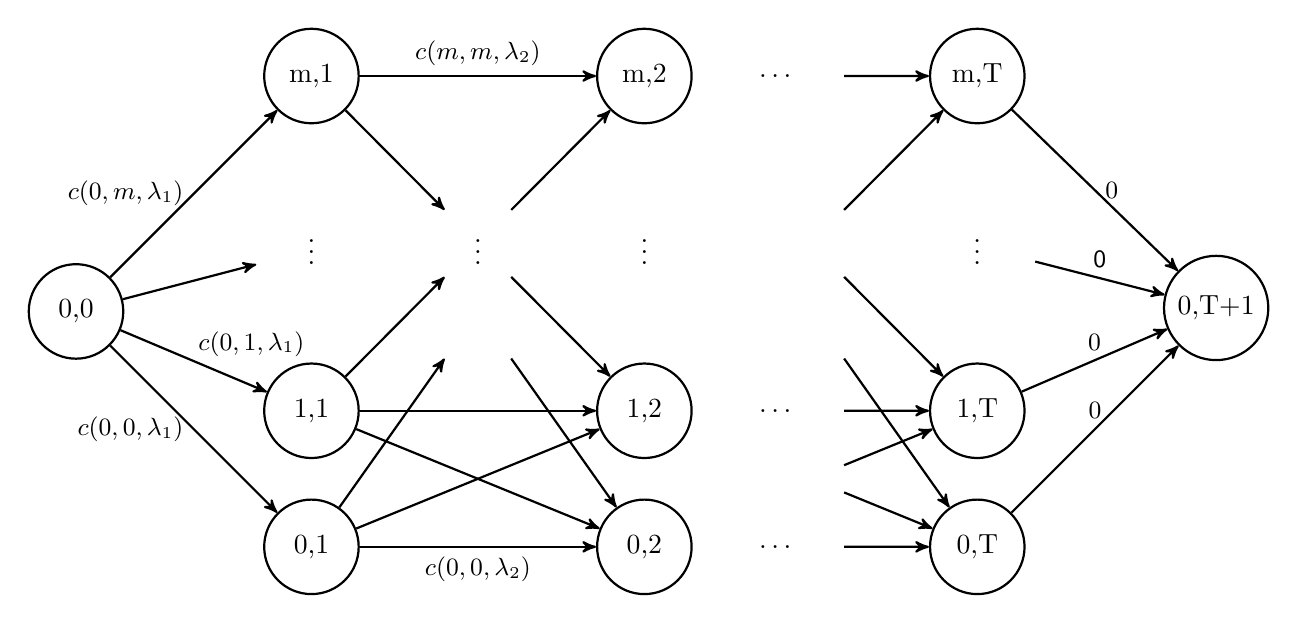
\begin{tikzpicture}[->,>=stealth',auto,node distance=3cm,thick,node/.style={minimum size=1.2cm,circle,draw}]

  \node[node] (1) {0,0};
  \node[node] (4) [below right =of 1] {0,1};
  \node[node] (3) [above =0.5cm of 4] {1,1};
  \node[node] (2) [above right=of 1] {m,1};
  \node[node] (6) [right =of 3] {1,2};
  \node[node] (5) [right =of 2] {m,2};
  \node[node] (7) [right =of 4] {0,2};
  \node[node] (9) [right =of 6] {1,T};
  \node[node] (8) [right =of 5] {m,T};
  \node[node] (10) [right =of 7] {0,T};
  \node[node] (11) [above right =of 10] {0,T+1};

  \node at ($(5)!.4!(8)$) {\ldots};
  \node at ($(6)!.4!(9)$) {\ldots};
  \node at ($(7)!.4!(10)$) {\ldots};

  \node at ($(2)!.5!(3)$) {\vdots};
  \node at ($(2)!.5!(6)$) {\vdots};
  \node at ($(5)!.5!(6)$) {\vdots};
  \node at ($(8)!.5!(9)$) {\vdots};

  \path[every node/.style={font=\sffamily\small}]
    (1) edge node[left] {$\costs(0,m,\lambda_1)$} (2)
	edge node[above right=-0.1cm] {$\costs(0,1,\lambda_1)$} (3)
	edge node[left] {$\costs(0,0,\lambda_1)$} (4)
    (2) edge node[above] {$\costs(m,m,\lambda_2)$} (5)
    (3) edge (6)
	edge (7)
    (4) edge (6)
	edge node[below] {$\costs(0,0,\lambda_2)$} (7)
    (8) edge node[right] {$0$} (11)
    (9) edge node[above] {$0$} (11)
    (10) edge node[above] {$0$} (11);

   \path [->,draw,thick] (1) to ($(1)!.2!(8)$);
   \path [->,draw,thick] (2) to ($(2)!.4!(6)$);
   \path [->,draw,thick] (4) to ($(4)!.4!(5)$);
   \path [->,draw,thick] (3) to ($(3)!.4!(5)$);

   \path [->,draw,thick] ($(3)!.6!(5)$) to (5);
   \path [->,draw,thick] ($(2)!.6!(6)$) to (6);
   \path [->,draw,thick] ($(2)!.6!(7)$) to (7);

   \path [->,draw,thick] ($(6)!.6!(8)$) to (8);
   \path [->,draw,thick] ($(5)!.6!(8)$) to (8);

   \path [->,draw,thick] ($(5)!.6!(9)$) to (9);
   \path [->,draw,thick] ($(6)!.6!(9)$) to (9);
   \path [->,draw,thick] ($(7)!.6!(9)$) to (9);

   \path [->,draw,thick] ($(5)!.6!(10)$) to (10);
   \path [->,draw,thick] ($(6)!.6!(10)$) to (10);
   \path [->,draw,thick] ($(7)!.6!(10)$) to (10);

   \path[every node/.style={font=\sffamily\small}] [->,draw,thick] ($(2)!.8!(11)$) -- node[above] {0} ++ (11);

\end{tikzpicture}
}
\caption{Level structured graph for an optimal offline algorithm.}
\end{figure}
We now want to verify the correctness of our construction.
\begin{prop}
	Any given optimal schedule $\mx$ corresponds to a shortest path $P$ from $(0,0)$ to $(T,0)$ with $costs(\mx)=costs(P)$ and vice versa.
\end{prop} 
\begin{proof}
$ $
\begin{itemize}
	\item[``$\Rightarrow$'':] We construct a feasible path in our graph from $\mx$ as follows:
\begin{align*}
	\text{First set}&&e_t&\coloneqq\Bigl(\bigl(t,\mx(t)\bigr),\bigl(t+1,\mx(t+1)\bigr)\Bigr),&\forall t\in\fromto{0}{T-1}\\
	\text{then set}&&P&\coloneqq(e_0,\ldots,e_{T-1})
\end{align*}
As each edge $e_t$ in our graph has weight $d\bigl(\mx(t-1),\mx(t),\lambda_{t}\bigr)$, it corresponds to the costs of switching from $\mx(t-1)$ to $\mx(t)$ servers and processing $\lambda_{t}$ with $\mx(t)$ active servers. Hence, it directly follows that $P$ is a shortest path of the graph with $costs(P)=costs(\mx)$.
	\item[``$\Leftarrow$'':] Let $P=\bigl((0,0)=v_0,\ldots,v_T=(T,0)\bigr)$ with $v_t\in\bigl\{(t,i)\mid 0\le i\le m\bigr\}$ be a shortest path of the graph.\\ 
	We can construct an optimal schedule from $P$ by setting $\mx\coloneqq\bigl(v_0(1),\ldots,v_T(1)\bigr)$\\
	By definition~\eqref{fct:c} it is guaranteed that $P$ only traverses edges such that there are enough active servers $\forall t\in[T]$. Therefore, the created schedule is feasible. Its optimality directly follows from the definition of the edges' weights and so does the equality $costs(\mx)=costs(P)$.
\end{itemize}
\end{proof}

\subsection{A pseudo-polynomial minimum cost algorithm}
\begin{algorithm}[H]
    \caption{Calculate costs for $m$ homogeneous servers}
    \begin{algorithmic}[1]
        \Require{Convex cost function $f$, $\lambda_0=\lambda_T=0$, $\forall t\in[T-1]:\lambda_t\in[0,m]$}
   \Function{schedule}{$m,T,\beta,\lambda_1,\ldots,\lambda_{T-1}$}
	\If{$T<2$} \Return
	\EndIf
	\Blet{$p[2\ldots T-1,m]$ and $M[1\ldots T-1,m]$}{new arrays}
	\For{$j \gets 0 \textrm{ to } m$}
		\Let{$M[1,j]$}{$d(0,j,\lambda_1)$}
	\EndFor
	\For{$t \gets 1 \textrm{ to } T-2$}
		\For{$j \gets 0 \textrm{ to } m$}
			\Let{$opt$}{$\infty$}
			\For{$i \gets 0 \textrm{ to } m$}
				\Let{$M[t+1,j]$}{$M[t,i]+d(i,j,\lambda_{t+1})$}
				\If{$M[t+1,j]<opt$}
					\Let{$opt$}{$M[t+1,j]$}
					\Let{$p[t+1,j]$}{$i$}
				\EndIf
			\EndFor
			\Let{$M[t+1,j]$}{$opt$}
		\EndFor
	\EndFor
	\State \Return{$p$ and $M$}
  \EndFunction
  \end{algorithmic}
\end{algorithm}
\begin{algorithm}[H]
    \caption{Extract schedule for $m$ homogeneous servers}
    \begin{algorithmic}[1]
   \Function{Extract}{$m,p,M,T$}
	\Blet{$x[0\ldots T]$}{a new array}
	\Let{$x[0]$}{$x[T]\leftarrow 0$}
	\If{$T<2$} \Return $x$ \Comment{Trivial solution}
	\EndIf
	\Let{$x[T-1]$}{$\underset{0\le i\le m}{arg\ min}\{M[T-1,i]\}$}
	\For{$t \gets T-2 \textrm{ to } 1$}
		\Let{$x[t]$}{$p[t+1,x[t+1]]$}
	\EndFor
	\State \Return{$x$}
  \EndFunction
  \end{algorithmic}
\end{algorithm}

\subsubsection{Runtime analysis}
The algorithm visits every vertex and every edge of the graph exactly once. As the number of vertices is bounded by $\mathcal{O}(Tm)$ and the number of edges is bounded by $\mathcal{O}(Tm^2)$ the running time is given by:
\begin{equation*}
	\mathcal{O}(Tm+Tm^2)=\mathcal{O}(Tm^2)
\end{equation*}
As we need $\log_2(m)$ bits to encode m, the running time is polynomial in the numeric value of the input but exponential in the length of the input. Hence, the algorithm is pseudo-polynomial.

\subsubsection{A memory optimized algorithm}
TODO: use only array with size 2m

\section{A polynomial $4$-approximation algorithm for monotonically increasing convex f}
We consider a modification of the problem discussed in chapter~\ref{sec:opt}. Assuming that f is convex and monotonically increasing, we can modify our algorithm to obtain a polynomial time $4$-approximation algorithm.

\subsection{Graph for a $4$-optimal schedule}
We modify our graph from chapter~\ref{sec:optgraph} to the reduce the number of vertices. For this, we stop adding m vertices for each timestep, but use vertices that approximate the number of active servers instead. First, let $b\coloneqq\lceil\log_2(m)\rceil$. We add vertices $(t,0)$ and $(t,2^i),\forall t\in[T-1],0\le i\le b$. All edges and weights are added analogous to chapter~\ref{sec:optgraph}.
\begin{figure}[H]
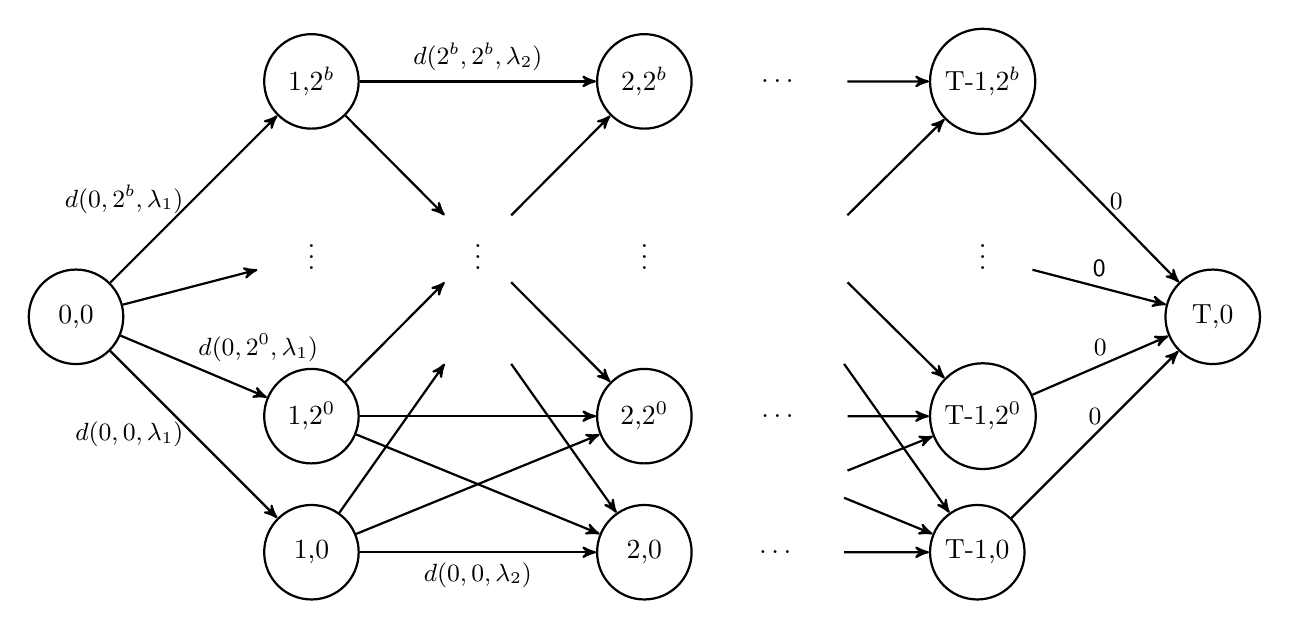
\begin{tikzpicture}[->,>=stealth',auto,node distance=3cm,thick,node/.style={minimum size=1.2cm,circle,draw}]

  \node[node] (1) {0,0};
  \node[node] (4) [below right =of 1] {1,0};
  \node[node] (3) [above =0.5cm of 4] {1,$2^0$};
  \node[node] (2) [above right=of 1] {1,$2^b$};
  \node[node] (6) [right =of 3] {2,$2^0$};
  \node[node] (5) [right =of 2] {2,$2^b$};
  \node[node] (7) [right =of 4] {2,0};
  \node[node] (9) [right =of 6] {T-1,$2^0$};
  \node[node] (8) [right =of 5] {T-1,$2^b$};
  \node[node] (10) [right =of 7] {T-1,0};
  \node[node] (11) [above right =of 10] {T,0};

  \node at ($(5)!.4!(8)$) {\ldots};
  \node at ($(6)!.4!(9)$) {\ldots};
  \node at ($(7)!.4!(10)$) {\ldots};

  \node at ($(2)!.5!(3)$) {\vdots};
  \node at ($(2)!.5!(6)$) {\vdots};
  \node at ($(5)!.5!(6)$) {\vdots};
  \node at ($(8)!.5!(9)$) {\vdots};

  \path[every node/.style={font=\sffamily\small}]
    (1) edge node[left] {$d(0,2^b,\lambda_1)$} (2)
	edge node[above right=-0.1cm] {$d(0,2^0,\lambda_1)$} (3)
	edge node[left] {$d(0,0,\lambda_1)$} (4)
    (2) edge node[above] {$d(2^b,2^b,\lambda_2)$} (5)
    (3) edge (6)
	edge (7)
    (4) edge (6)
	edge node[below] {$d(0,0,\lambda_2)$} (7)
    (8) edge node[right] {$0$} (11)
    (9) edge node[above] {$0$} (11)
    (10) edge node[above] {$0$} (11);

   \path [->,draw,thick] (1) to ($(1)!.2!(8)$);
   \path [->,draw,thick] (2) to ($(2)!.4!(6)$);
   \path [->,draw,thick] (4) to ($(4)!.4!(5)$);
   \path [->,draw,thick] (3) to ($(3)!.4!(5)$);

   \path [->,draw,thick] ($(3)!.6!(5)$) to (5);
   \path [->,draw,thick] ($(2)!.6!(6)$) to (6);
   \path [->,draw,thick] ($(2)!.6!(7)$) to (7);

   \path [->,draw,thick] ($(6)!.6!(8)$) to (8);
   \path [->,draw,thick] ($(5)!.6!(8)$) to (8);

   \path [->,draw,thick] ($(5)!.6!(9)$) to (9);
   \path [->,draw,thick] ($(6)!.6!(9)$) to (9);
   \path [->,draw,thick] ($(7)!.6!(9)$) to (9);

   \path [->,draw,thick] ($(5)!.6!(10)$) to (10);
   \path [->,draw,thick] ($(6)!.6!(10)$) to (10);
   \path [->,draw,thick] ($(7)!.6!(10)$) to (10);

   \path[every node/.style={font=\sffamily\small}] [->,draw,thick] ($(2)!.8!(11)$) -- node[above] {0} ++ (11);

\end{tikzpicture}
\caption{Graph for a $4$-approximation algorithm}
\end{figure}

\begin{defn}
Let $\mx=(x_0,\ldots,x_T)$ be a schedule and $t>0$.\\
We say that $\mx$ changes its \textbf{state} at time t if
\begin{equation*}
	x_t\neq x_{t-1}
\end{equation*}
and that $\mx$ changes its \textbf{2-state} at time t if
\begin{equation*}
	x_t=0\text{\quad or\quad}x_t\notin\bigl(2^{\lfloor \log_2(x_{t-1})\rfloor},2^{\lceil \log_2(x_{t-1})\rceil}\bigr)
\end{equation*}
\end{defn}
\begin{prop}
$ $
\begin{enumerate}
	\item\label{prop:2opt} Any given optimal schedule $\mx$ can be transformed to a $4$-optimal schedule $\mx'$ which corresponds to a path $P$ from $(0,0)$ to $(T,0)$ with $costs(\mx')=costs(P)$.
	\item Any shortest path $P$ from $(0,0)$ to $(T,0)$ corresponds to a $4$-optimal schedule $\mx$ with $costs(P)=costs(\mx)$.
\end{enumerate}
\end{prop}
\begin{proof}
$ $
\begin{enumerate}
	\item Assume we have an optimal schedule identified by $\mx=(x_0,\ldots,x_T)$. For $0\le t<T$ we inductively set:
\begin{equation}
	x'_0\coloneqq 0,\qquad
	x'_{t+1}\coloneqq 
	\begin{cases}
		\min\bigl\{2^{\lfloor \log_2(2x_{t+1})\rfloor},2^b\bigr\}, & \text{if $0<x_t\le x_{t+1}$}\\
		2^{\lceil \log_2(2x_{t+1})\rceil}, & \text{if $0<x_{t+1}<x_t$ and $x'_{t}\ge4x_{t+1}$}\\
		x'_t, & \text{if $0<x_{t+1}<x_t$ and $x'_{t}<4x_{t+1}$}\\
		\		   0, & \text{otherwise}
	\end{cases} \label{def:chi_prime}
\end{equation}
Then let $\mx'\coloneqq(x'_0,\ldots,x'_T)$ be the modified sequence of active servers. Notice that \makebox{$x_t\le x'_t\le 4x_t$} holds as $x'_t$ is at most the smallest power of two larger than $2x_t$ which implies that $\mx'$ is feasible.\\
We can now construct a feasible path in our graph from $\mathcal{X'}$ as follows:
\begin{align*}
	\text{First set}&&e_t&\coloneqq\Bigl(\bigl(t,\mx'(t)\bigr),\bigl(t+1,\mx'(t+1)\bigr)\Bigr),&\forall t\in\fromto{0}{T-1}\\
	\text{then set}&&P&\coloneqq(e_0,\ldots,e_{T-1})
\end{align*}
By the definition of the edges' weights it follows that $costs(\mx')=costs(P)$.\\
Next, let $(t_0=0,t_1,\ldots,t_n=0)$ be the sequence of times where the optimal schedule $\mx$ changes its 2-state. Notice that the modified schedule $\mx'$ changes its state only at times $t_i$ and that $2x_{t_i}\le x'_{t_i}$ holds (TODO: only if not discrete but continous time steps). This can be seen exemplarily in figure~\ref{fig:adaption-schedule} by obvserving that $\mx'$ changes its state only if $\mx$ crosses or touches a bordering power of two.
\begin{figure}[H]
\centering
\scalebox{0.7}{
\subfloat{
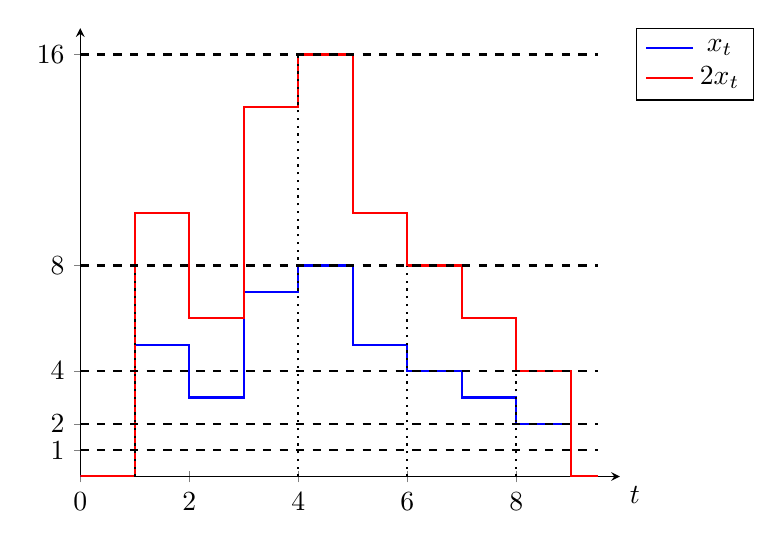
\begin{tikzpicture}
	\begin{axis}[%
	    ,xlabel=$t$
	    ,axis x line = bottom,axis y line = left
	    ,ytick={1,2,4,8,16}
	    ,ymax=17 % or enlarge y limits=upper
	    ,xmax=9.9
	    ,legend pos=outer north east
	    ]
	\addplot+[const plot, no marks, thick, color=blue] coordinates {(0,0) (1,5) (2,3) (3,7) (4,8) (5,5) (6,4) (7,3) (8,2) (9,0) (9.5,0)};
	\addplot+[const plot, no marks, thick, color=red] coordinates {(0,0) (1,10) (2,6) (3,14) (4,16) (5,10) (6,8) (7,6) (8,4) (9,0) (9.5,0)};
	\addplot+[const plot, no marks, thick, dotted, color=black] coordinates {(1,0) (1,8)};
	\addplot+[const plot, no marks, thick, dotted, color=black] coordinates {(4,0) (4,16)};
	\addplot+[const plot, no marks, thick, dotted, color=black] coordinates {(6,0) (6,8)};
	\addplot+[const plot, no marks, thick, dotted, color=black] coordinates {(8,0) (8,4)};
	\addplot+[const plot, no marks, thick, dashed, color=black] coordinates {(0,1) (9.5,1)};
	\addplot+[const plot, no marks, thick, dashed, color=black] coordinates {(0,2) (9.5,2)};
	\addplot+[const plot, no marks, thick, dashed, color=black] coordinates {(0,4) (9.5,4)};
	\addplot+[const plot, no marks, thick, dashed, color=black] coordinates {(0,8) (9.5,8)};
	\addplot+[const plot, no marks, thick, dashed, color=black] coordinates {(0,16) (9.5,16)};
	\addlegendentry{$x_t$}
	\addlegendentry{$2x_t$}
	\end{axis}
\end{tikzpicture}}}
\qquad
\scalebox{0.7}{
\subfloat{
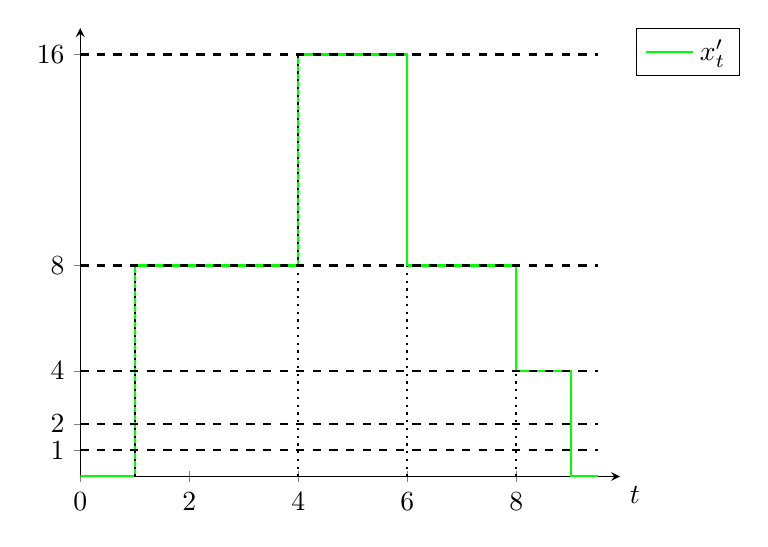
\begin{tikzpicture}
	\begin{axis}[%
	    ,xlabel=$t$
	    ,axis x line = bottom,axis y line = left
	    ,ytick={1,2,4,8,16}
	    ,ymax=17 % or enlarge y limits=upper
	    ,xmax=9.9
	    ,legend pos=outer north east
	    ]
	\addplot+[const plot, no marks, thick, color=green] coordinates {(0,0) (1,8) (2,8) (3,8) (4,16) (5,16) (6,8) (7,8) (8,4) (9,0) (9.5,0)};
	\addplot+[const plot, no marks, thick, dotted, color=black] coordinates {(1,0) (1,8)};
	\addplot+[const plot, no marks, thick, dotted, color=black] coordinates {(4,0) (4,16)};
	\addplot+[const plot, no marks, thick, dotted, color=black] coordinates {(6,0) (6,8)};
	\addplot+[const plot, no marks, thick, dotted, color=black] coordinates {(8,0) (8,4)};
	\addplot+[const plot, no marks, thick, dashed, color=black] coordinates {(0,1) (9.5,1)};
	\addplot+[const plot, no marks, thick, dashed, color=black] coordinates {(0,2) (9.5,2)};
	\addplot+[const plot, no marks, thick, dashed, color=black] coordinates {(0,4) (9.5,4)};
	\addplot+[const plot, no marks, thick, dashed, color=black] coordinates {(0,8) (9.5,8)};
	\addplot+[const plot, no marks, thick, dashed, color=black] coordinates {(0,16) (9.5,16)};
	\addlegendentry{$x'_t$}
	\end{axis}
\end{tikzpicture}}}
 	\caption{Adaption of an optimal schedule}
	\label{fig:adaption-schedule}
\end{figure}
	For this reason, we now only have to consider the fraction of costs of $\mx'$ and $\mx$ between time steps $t_{i-1}$ and $t_i$
	\begin{equation}
		\frac{costs(\mx',t_{i-1},t_i)}{costs(\mx,t_{i-1},t_i)}\label{eq:frac_chi_prime}
	\end{equation}
	For $x_{t_i}=0$ it follows from \eqref{eq:costs_chi_t_t_prime} that $costs(\mx',t_{i-1},t_i)=costs(\mx,t_{i-1},t_i)=0$. Hence, we can restrict ourselves to $0<t_i<T$ with $x_{t_i}\neq 0$.
	The costs incurred by $\mx'$ are given by
	\begin{align}
		&&costs(\mx',t_{i-1},t_i)&=\beta\max\{0,x'_{t_i}-x'_{t_{i-1}}\}+x'_{t_i}f(\lambda_{t_i}/x'_{t_i})&\text{by \eqref{eq:costs_chi_t_t_prime}}\nonumber\\
		&&&\le\beta\max\{0,x'_{t_i}-x'_{t_{i-1}}\}+4x_{t_i}f(\lambda_{t_i}/x'_{t_i})&\text{by \eqref{def:chi_prime}}\nonumber\\
		&&&\le\beta\max\{0,x'_{t_i}-x'_{t_{i-1}}\}+4x_{t_i}f(\lambda_{t_i}/x_{t_i})&\text{f monotonically increasing}\nonumber\\
		\implies&&costs(\mx',t_{i-1},t_i)&\le\beta\max\{0,x'_{t_i}-x'_{t_{i-1}}\}+4x_{t_i}f(\lambda_{t_i}/x_{t_i})\label{eq:est_chi_prime}
	\end{align}
	and the costs of $\mx$ by
	\begin{equation}
		costs(\mx,t_{i-1},t_i)=\beta\max\{0,x_{t_i}-x_{t_{i-1}}\}+x_{t_i}f(\lambda_{t_i}/x_{t_i})\label{eq:optcosts}
	\end{equation}
	W.l.o.g.\ we may assume $x_{t_i}f(\lambda_{t_i}/x_{t_i})>0$, otherwise the claim follows trivially. (TODO: is it really trivial?)
	\begin{enumerate}[(i)]
		\item\label{pr:4appr_1} \underline{$x_{t_i}\le x_{t_{i-1}}$:}
			From~\eqref{def:chi_prime} it follows that $x'_{t_i}\le x'_{t_{i-1}}$. Thus, we can simplify~\eqref{eq:frac_chi_prime}:
		\begin{align*}
			\frac{costs(\mx',t_{i-1},t_i)}{costs(\mx,t_{i-1},t_i)}&\le\frac{\beta\max\{0,x'_{t_i}-x'_{t_{i-1}}\}+4x_{t_i}f(\lambda_{t_i}/x_{t_i})}{\beta\max\{0,x_{t_i}-x_{t_{i-1}}\}+x_{t_i}f(\lambda_{t_i}/x_{t_i})}&\text{by \eqref{eq:est_chi_prime},\eqref{eq:optcosts}}\\
			&=\frac{4x_{t_i}f(\lambda_{t_i}/x_{t_i})}{x_{t_i}f(\lambda_{t_i}/x_{t_i})}&\text{($x_{t_i}\le x_{t_{i-1}}$ and $x'_{t_i}\le x'_{t_{i-1}}$)}\\
			&=4
		\end{align*}
		\item\label{pr:4appr_2} \underline{$x_{t_i}>x_{t_{i-1}}$:}
		From (\ref{def:chi_prime}) it follows that $x'_{t_i}\ge x'_{t_{i-1}}$. Thus, we can simplify~(\ref{eq:frac_chi_prime}):
		\begin{align*}
			\frac{costs(\mx',t_{i-1},t_i)}{costs(\mx,t_{i-1},t_i)}&\le\frac{\beta\max\{0,x'_{t_i}-x'_{t_{i-1}}\}+4x_{t_i}f(\lambda_{t_i}/x_{t_i})}{\beta\max\{0,x_{t_i}-x_{t_{i-1}}\}+x_{t_i}f(\lambda_{t_i}/x_{t_i})}&\text{by \eqref{eq:est_chi_prime},\eqref{eq:optcosts}}\\
			&=\frac{\beta(x'_{t_i}-x'_{t_{i-1}})+4x_{t_i}f(\lambda_{t_i}/x_{t_i})}{\beta(x_{t_i}-x_{t_{i-1}})+x_{t_i}f(\lambda_{t_i}/x_{t_i})}&\text{($x_{t_i}>x_{t_{i-1}}$ and $x'_{t_i}\ge x'_{t_{i-1}}$)}\\
			&=\frac{\beta(\min\bigl\{2^{\lfloor \log_2(2x_{t_i})\rfloor},2^b\bigr\}-x'_{t_{i-1}})+4x_{t_i}f(\lambda_{t_i}/x_{t_i})}{\beta(x_{t_i}-x_{t_{i-1}})+x_{t_i}f(\lambda_{t_i}/x_{t_i})}&\text{by \eqref{def:chi_prime}}\\
			&\le\frac{\beta(2^{\lfloor \log_2(2x_{t_i})\rfloor}-x'_{t_{i-1}})+4x_{t_i}f(\lambda_{t_i}/x_{t_i})}{\beta(x_{t_i}-x_{t_{i-1}})+x_{t_i}f(\lambda_{t_i}/x_{t_i})}\\
			&\le\frac{\beta(2x_{t_i}-x'_{t_{i-1}})+4x_{t_i}f(\lambda_{t_i}/x_{t_i})}{\beta(x_{t_i}-x_{t_{i-1}})+x_{t_i}f(\lambda_{t_i}/x_{t_i})}\\
			&\le\frac{\beta(2x_{t_i}-2x_{t_{i-1}})+4x_{t_i}f(\lambda_{t_i}/x_{t_i})}{\beta(x_{t_i}-x_{t_{i-1}})+x_{t_i}f(\lambda_{t_i}/x_{t_i})}&\text{by ($2x_{t_{i-1}}\le x'_{t_{i-1}}$)}\\
			&\le4\ \frac{\frac{1}{2}\beta(x_{t_i}-x_{t_{i-1}})+x_{t_i}f(\lambda_{t_i}/x_{t_i})}{\ \ \beta(x_{t_i}-x_{t_{i-1}})+x_{t_i}f(\lambda_{t_i}/x_{t_i})}\\
			&\le4
		\end{align*}
	\end{enumerate}
	From~(\hyperref[pr:4appr_1]{i}) and~(\hyperref[pr:4appr_2]{ii}) it follows:
	\begin{equation*}
		costs(\mx')\le4costs(\mx)
	\end{equation*}
	\item From~\ref{prop:2opt} we obtain that we can construct a $4$-optimal path $P'$ from any optimal schedule. Now, let $P$ be a shortest path. We have $costs(P)\le costs(P')<\infty$, and since every path $P$ with $costs(P)<\infty$ corresponds to a feasible schedule $\mx$ with $costs(P)=costs(\mx)$, $\mx$ must also be at least $4$-optimal.
\end{enumerate}
\end{proof}

\newpage
\bibliographystyle{plain}
\bibliography{sources.bib}
\newpage

\section*{Appendix}
Below, we give an overview of just given definitions and conventions commonly referred to in our paper:\unsure{Good idea to have an appendix?}
%\scriptsize
%\begin{multicols}{2}
\begin{itemize}
\item Input:
\begin{itemize}
	\item $m\in\mathbb{N}$\ldots number of homogeneous servers
	\item $T\in\mathbb{N}$\ldots number of time slots
	\item $\lambda_1,\ldots,\lambda_{T}\in[0,m]$\ldots arrival rates
	\item $\Lambda\coloneqq(\lambda_1,\ldots,\lambda_T)$\ldots sequence of arrival rates
	\item $\beta\in\mathbb{R}_{\ge 0}$\ldots switching costs of a server
	\item $f:[0,1]\rightarrow\mathbb{R}$\ldots convex operating costs function of a server
	\item $\inp\coloneqq(m,T,\Lambda,\beta,f)$\ldots input of a problem instance
\end{itemize}

\item Problem statement:
\begin{itemize}
	\item $s_{i,t}$\ldots state of server $i$ at time $t$, i.e.\ sleeping (0) or active(1)
	\item $S_i\coloneqq(s_{i,1},\ldots,s_{i,T})\in\{0,1\}^T$\ldots sequence of states for server $i$
	\item $\lambda_{i,t}\in[0,1]$\ldots assigned load for server $i$ at time $t$
	\item $L_i\coloneqq(\lambda_{i,1},\ldots,\lambda_{i,T})\in[0,1]^T$\ldots sequence of assigned loads for server $i$
	\item $\mathcal{S}\coloneqq(S_1,\ldots,S_m)$\ldots sequence of all state changes
	\item $\mathcal{L}\coloneqq(L_1,\ldots,L_m)$\ldots sequence of all assigned loads
	\item $\Sigma\coloneqq(\mathcal{S},\mathcal{L})$\ldots schedule for a problem instance $\inp$
\end{itemize}

\item Miscellaneous:
\begin{itemize}
	\item $x_t$\ldots number of active servers at time t
	\item $\mx\coloneqq(x_1,\ldots,x_T)$\ldots sequence of number of active servers
\end{itemize}

\item Conventions:
\begin{itemize}
	\item $\lambda_{t}=0$ for all $t\notin[T]$, i.e.\ there is no load before and after the scheduling process
	\item $s_{i,t}=0$ for all $t\notin[T]$, i.e.\ all servers are powered down before and after the scheduling process
\end{itemize}
\end{itemize}
%\end{multicols}
\normalsize

\end{document}
